\section{Introdução}
Na engenharia, é essencial abordar problemas físicos que emergem de sistemas descritos por equações diferenciais. Esses problemas podem ser tratados de diversas maneiras, dependendo das ferramentas disponíveis e da natureza específica do desafio. Analogamente, pode-se comparar a formação em engenharia a uma caixa de ferramentas: o curso representa a caixa, enquanto as disciplinas e seus conteúdos são as ferramentas disponíveis. Cabe ao engenheiro escolher a ferramenta mais adequada para cada situação, considerando suas vantagens e limitações.

Para modelar matematicamente esses problemas físicos, é necessário traduzir fenômenos reais em expressões matemáticas, muitas das quais são equações diferenciais. Com essas expressões, pode-se modelar sistemas e aplicar uma variedade de métodos analíticos e computacionais para interpretá-los e controlá-los.

No contexto dos problemas físicos que requerem controle, sistemas de controle são essenciais para obter respostas específicas desejadas. Nesses sistemas, uma entidade conhecida como planta física interage com uma controladora. A controladora, auxiliada por sensores, ajusta suas ações baseada na resposta que monitora, visando manter o sistema dentro de parâmetros desejados. Um exemplo típico desses sistemas é um aquecedor controlado automaticamente, que utiliza sensores para manter uma temperatura ambiente constante.

Os sistemas podem ser categorizados como de malha aberta, quando não há feedback de controle, e de malha fechada, quando o sistema de controle ajusta dinamicamente a operação baseando-se no feedback recebido. A figura 1 ilustra de maneira generalizada um sistema de malha aberta.


Na engenharia, a capacidade de modelar e controlar sistemas dinâmicos é crucial para o desenvolvimento de soluções eficazes para problemas reais. Sistemas descritos por equações diferenciais, como o sistema massa-mola-amortecedor ilustrado abaixo, são exemplos fundamentais nesse contexto. Este sistema é um modelo clássico usado para entender como as forças são transmitidas e modificadas em sistemas mecânicos.

\begin{figure}[H]
    \centering
    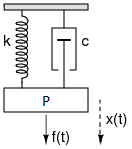
\includegraphics[width=0.3\textwidth]{main/introducao/assets/modelagem.png}
    \caption{Sistema massa-mola-amortecedor}
    \label{fig:modelagem}
\end{figure}

O sistema consiste em uma massa \( m \), uma mola com constante \( k \), e um amortecedor com coeficiente \( c \), todos configurados como mostrado na figura. A força aplicada \( f(t) \) e o deslocamento da massa \( x(t) \) são relacionados pela seguinte equação diferencial:

\[
    f(t) = m \frac{d^2x(t)}{dt^2} + c \frac{dx(t)}{dt} + kx(t)
\]
Esta equação modela a força necessária para mover a massa, considerando a inércia do objeto, a resistência proporcionada pelo amortecedor e a força restauradora da mola. O termo \( m \frac{d^2x(t)}{dt^2} \) representa a força inercial, \( c \frac{dx(t)}{dt} \) representa a força de amortecimento que é proporcional à velocidade, e \( kx(t) \) é a força restauradora da mola que é proporcional ao deslocamento.

Estudar esse sistema permite compreender como diferentes parâmetros influenciam o comportamento dinâmico, facilitando a aplicação de técnicas de controle para alcançar um desempenho desejado. Além disso, a modelagem matemática e a simulação computacional com ferramentas como o Scilab e o Xcos são fundamentais para analisar e prever o comportamento de sistemas complexos, proporcionando um entendimento profundo e a capacidade de desenvolver soluções inovadoras.

Neste trabalho, focaremos na análise de sistemas de controle de malha fechada, utilizando o modelo massa-mola-amortecedor. Serão abordadas resoluções de problemas específicos para os valores de \( M = 10 \), \( C = 7 \), e \( k = 5 \), demonstrando como ajustar os parâmetros de controle para otimizar a resposta do sistema.
